\documentclass[border=2mm]{standalone}
\usepackage{pgfplots}
\pgfplotsset{compat=1.8}
\begin{document}
\newcommand\bhone {(3.0,0.0,0.0)}
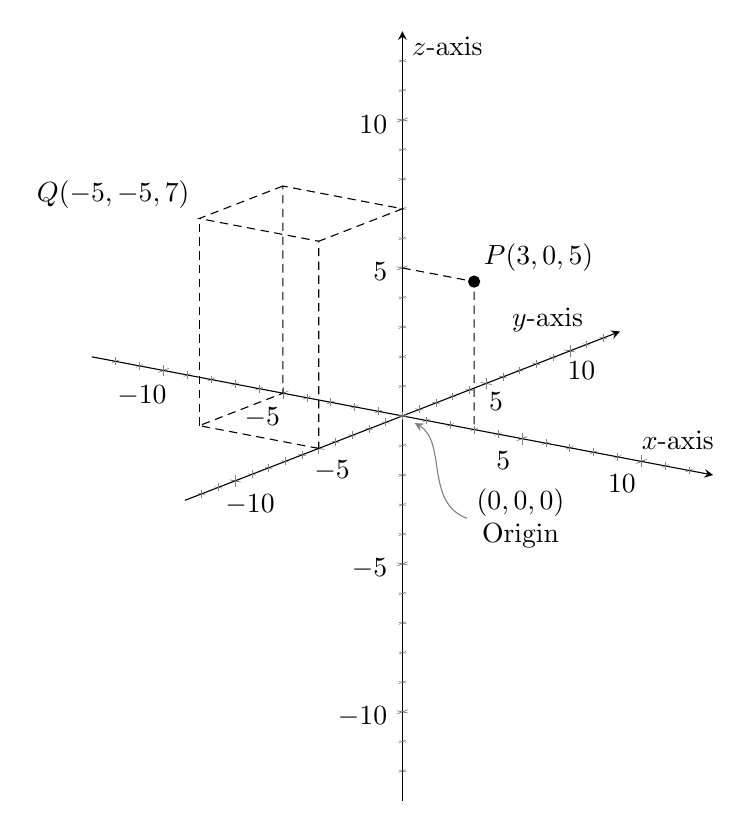
\begin{tikzpicture}
\begin{axis}[
  view={35}{15},
  axis lines=center,
  width=15cm,height=15cm,
  xtick={-10,-5,5,10},ytick={-10,-5,5,10},ztick={-10,-5,5,10},
  minor tick={-12,-11,...,12},
  xmin=-13,xmax=13,ymin=-13,ymax=13,zmin=-13,zmax=13,
  xlabel={$x$-axis},ylabel={$y$-axis},zlabel={$z$-axis},
]




% plot dots for the two points
\addplot3 [only marks] coordinates {\bhone (3,0,5)};

% plot dashed lines to axes
\addplot3 [no marks,densely dashed] coordinates {(0,0,5) (3,0,5) (3,0,0)};
\addplot3 [no marks,densely dashed] coordinates {(0,-5,0) (-5,-5,0) (-5,0,0) (-5,0,7) (0,0,7) (0,-5,7) (0,-5,0)};
\addplot3 [no marks,densely dashed] coordinates {(-5,0,7) (-5,-5,7) (0,-5,7)};
\addplot3 [no marks,densely dashed] coordinates {(-5,-5,0) (-5,-5,7)};

% label points
\node [above right] at (axis cs:3,0,5) {$P (3,0,5)$};
\node [above left] at (axis cs:-5,-5,7) {$Q (-5,-5,7)$};
\node [inner sep=2pt,outer sep=0pt] (O) at (axis cs:0,0,0) {};
\node [align=center] (origin) at ([xshift=1.5cm,yshift=-1.3cm]O) {$(0,0,0)$ \\Origin};
\draw [shorten <=.1cm,stealth-,gray] (O) to [out=-30,in=160] (origin.west);
\end{axis}
\end{tikzpicture}
\end{document}
